\documentclass[a4paper]{article}

\usepackage[english]{babel}
\usepackage[utf8]{inputenc}
\usepackage{csquotes}
\usepackage{amsmath, latexsym}
\usepackage{graphicx}
\usepackage{tikz}
\usepackage{listings}
\usepackage{verbatim}
\usepackage{bigints}
\usepackage{float}
\usepackage{titling}
\usepackage[colorinlistoftodos]{todonotes}
\usepackage[style=authoryear,sorting=nty,maxcitenames=1]{biblatex}



\title{Computational study of far-field acoustic emission by collapsing bubbles}
\author{}
\date{\today}
\addbibresource{references.bib}



\begin{document}
\maketitle
\section{Kirchhoff formulation}
\begin{figure}[h!]\label{Kirchhoff}
	\centering
	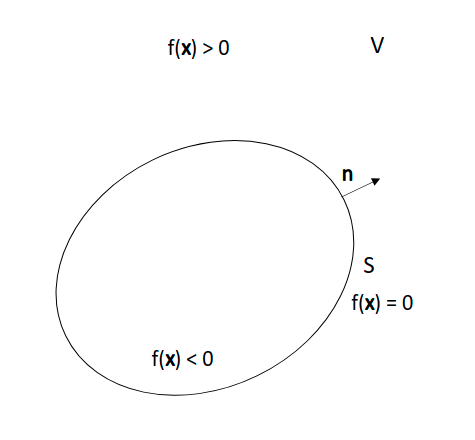
\includegraphics[width=60mm]{images/kirchhoff_surface.png}
	\caption{Stationary Kirchhoff surface $S$ encloses sound source}
\end{figure}
In this section, we derive the Kirchhoff formula for a stationary control surface (\cite{FARASSAT1988451}). We chose a control surface $S$ that encloses all the acoustic sources (\ref{Kirchhoff}), and the pressure perturbations $p$ satisfies the homogeneous wave equation
\begin{equation}\label{Wave equation}
	\Bigg( \frac{1}{c_{0}^2}\frac{\partial{}^{2}}{\partial{t}^{2}}- \nabla{}^{2} \Bigg) p = 0 \quad \quad \textrm{in} \ V.
\end{equation}
The control surface S is defined by $f(\mathbf{x}) = 0$, $f(\mathbf{x}) > 0$ for $\mathbf{x}$ in V and $f(\mathbf{x}) < 0$ for $\mathbf{x}$ inside surface S. We scale the function $f$ such that $\nabla f = \mathbf{n}$. Then the Heaviside function of $f(\mathbf{x})$    is
\begin{equation}\label{Heaviside}
	H(f) =\begin{cases}
		1, & \text{for $\mathbf{x}$ in V}.     \\
		0, & \text{for $\mathbf{x}$ inside S}.
	\end{cases}
\end{equation}
The gradient of the Heaviside function is given by
\begin{equation}\label{Gradient Heaviside}
	\nabla H(f) = \delta (f) \mathbf{n}.
\end{equation}
We define the pressure $p$ as a generalized function $pH(f)$ (\cite{ffowcs1969sound}) where
\begin{equation}\label{Generalized_Functions}
	p H(f) =\begin{cases}
		p , & \text{for $\mathbf{x}$ in V}.     \\
		0,  & \text{for $\mathbf{x}$ inside S}.
	\end{cases}
\end{equation}
The generalized pressure $pH(f)$ is defined everywhere in space, unlike $p$ defined only in $V$. We will derive the acoustic wave equation for the generalised pressure. Using (\ref{Gradient Heaviside}), the gradient of $pH$ is
\begin{equation}
	\nabla (pH) = \nabla p H + p \delta(f)\mathbf{n}.
\end{equation}
Therefor the Laplacian is given by
\begin{equation}\label{Laplacian}
	\nabla^2 (pH) = \nabla^2 p H +  \frac{\partial p}{\partial n}\delta(f) + \nabla.(p \delta(f)\mathbf{n}).
\end{equation}
The partial derivative in time is
\begin{equation}\label{Time derivative}
	\frac{\partial^2}{\partial t^2}(pH) = \frac{\partial^2 p }{\partial t^2}H.
\end{equation}
We premultiply (\ref{Time derivative}) with $1/{c_{0}^2}$ and subtract (\ref{Laplacian}) to obtain the acoustic wave equation in generalised pressure
\begin{equation}
	\Bigg( \frac{1}{c_{0}^2}\frac{\partial{}^{2}}{\partial{t}^{2}}- \nabla{}^{2} \Bigg) pH = H\Bigg( \frac{1}{c_{0}^2}\frac{\partial{}^{2}}{\partial{t}^{2}}- \nabla{}^{2} \Bigg) p - \frac{\partial p}{\partial n}\delta(f) - \nabla.(p \delta(f)\mathbf{n}),
\end{equation}
or
\begin{equation}\label{Generalized Wave Equation}
	\Bigg( \frac{1}{c_{0}^2}\frac{\partial{}^{2}}{\partial{t}^{2}}- \nabla{}^{2} \Bigg) pH = -\frac{\partial p}{\partial n}\delta(f) - \nabla.(p \mathbf{n} \delta(f)).
\end{equation}
The right side of the equation (\ref{Generalized Wave Equation}) is non-zero only at surface $S$, as it contains $\delta (f)$. The acoustic wave equation (\ref{Generalized Wave Equation}) in generalized variables is valid in the entire unbounded space. Therefore we can use free-space Green's function to solve the equation. The Green's function is the solution of wave equation for an impulsive point source $\delta(\mathbf{x} - \mathbf{y})\delta(t - \tau)$ placed at point $\mathbf{y}$ and time $\tau$
\begin{equation}\label{green}
	\Bigg( \frac{1}{c_{0}^2}\frac{\partial{}^{2}}{\partial{t}^{2}}- \nabla{}^{2} \Bigg){G(\mathbf{x}, t; \mathbf{y}, \tau )} = \delta{(\mathbf{x} - \mathbf{y})}\delta{(t - \tau)}.
\end{equation}
The Green's function for the acoustic wave operator (\cite{howe2003theory}) in three dimensions is
\begin{equation}\label{Green's Function}
	G(\mathbf{x}, t; \mathbf{y}, \tau ) = \frac{\delta \Big(t - \tau - \frac{|\mathbf{x} - \mathbf{y}|}{c_{0}}\Big)}{4\pi|\mathbf{x} - \mathbf{y}|}.
\end{equation}
The solution for arbirtary source can be obtained by multiplying $s(\mathbf{y}, \tau)$ in (\ref{green})
\begin{equation}
	\Bigg( \frac{1}{c_{0}^2}\frac{\partial{}^{2}}{\partial{t}^{2}}- \nabla{}^{2} \Bigg)s(\mathbf{y}, \tau){G(\mathbf{x}, t; \mathbf{y}, \tau )} = s(\mathbf{y}, \tau)\delta{(\mathbf{x} - \mathbf{y})}\delta{(t - \tau)},
\end{equation}
Integrating both sides
\begin{equation}
	\Bigg( \frac{1}{c_{0}^2}\frac{\partial{}^{2}}{\partial{t}^{2}}- \nabla{}^{2} \Bigg) \int s(\mathbf{y}, \tau){G(\mathbf{x}, t; \mathbf{y}, \tau )} d\mathbf{y}d\tau  = \int s(\mathbf{y}, \tau)\delta{(\mathbf{x} - \mathbf{y})}\delta{(t - \tau)} d\mathbf{y}d\tau,
\end{equation}
and using the properties of delta function, we get the solution for the acoustic wave equation with source $s(\mathbf{x}, t)$
\begin{equation}
	\Bigg( \frac{1}{c_{0}^2}\frac{\partial{}^{2}}{\partial{t}^{2}}- \nabla{}^{2} \Bigg) p(\mathbf{x}, t)  = s(\mathbf{x}, t),
\end{equation}
where,
\begin{equation}\label{pressure}
	p(\mathbf{x}, t) = \int s(\mathbf{y}, \tau){G(\mathbf{x}, t; \mathbf{y}, \tau )} d\mathbf{y}d\tau.
\end{equation}
We can use the above relation to solve the acoustic wave equation (\ref{Generalized Wave Equation})
\begin{equation}
	\begin{split}
		(pH)(\mathbf{x}, t) = &-\frac{1}{4\pi}\int {\frac{\partial p}{\partial n}\delta(f) \frac{\delta \Big(t - \tau - \frac{|\mathbf{x} - \mathbf{y}|}{c_{0}}\Big)}{|\mathbf{x} - \mathbf{y}|}} d\mathbf{y}d\tau \\
		&-\frac{1}{4\pi}\int \nabla_{\mathbf{y}}.(p \mathbf{n} \delta(f)){\frac{\delta \Big(t - \tau - \frac{|\mathbf{x} - \mathbf{y}|}{c_{0}}\Big)}{|\mathbf{x} - \mathbf{y}|}} d\mathbf{y}d\tau.
	\end{split}
\end{equation}
\begin{equation}
	\begin{split}
		(pH)(\mathbf{x}, t) = &-\frac{1}{4\pi}\int {\frac{\partial p}{\partial n}\delta(f) \frac{\delta \Big(t - \tau - \frac{|\mathbf{x} - \mathbf{y}|}{c_{0}}\Big)}{|\mathbf{x} - \mathbf{y}|}} d\mathbf{y}d\tau \\
		&-\frac{1}{4\pi}\nabla_{\mathbf{x}}.\int (p \mathbf{n} \delta(f)){\frac{\delta \Big(t - \tau - \frac{|\mathbf{x} - \mathbf{y}|}{c_{0}}\Big)}{|\mathbf{x} - \mathbf{y}|}} d\mathbf{y}d\tau.
	\end{split}
\end{equation}
We use the following property to convert volume integral to surface integral (\cite{FARASSAT1988451}).
\begin{equation}\label{volume surface}
	\int \phi (\mathbf{y}) \delta (f) \mathbf{n} d\mathbf{y} = \int_{S} \phi (\mathbf{y}) \mathbf{n} dS
\end{equation}
We use the above property to convert volume integral to surface integral on $S$
\begin{equation}
	\begin{split}
		(pH)(\mathbf{x}, t) = &-\frac{1}{4\pi}\int {\frac{\partial p}{\partial n} \frac{\delta \Big(t - \tau - \frac{|\mathbf{x} - \mathbf{y}|}{c_{0}}\Big)}{|\mathbf{x} - \mathbf{y}|}} dSd\tau \\
		&-\frac{1}{4\pi}\nabla_{\mathbf{x}}.\int (p \mathbf{n} ){\frac{\delta \Big(t - \tau - \frac{|\mathbf{x} - \mathbf{y}|}{c_{0}}\Big)}{|\mathbf{x} - \mathbf{y}|}} dSd\tau.
	\end{split}
\end{equation}
Using the property of delta function we obtain
\begin{equation}
	\begin{split}
		(pH)(\mathbf{x}, t) = &-\frac{1}{4\pi}\int_{S} { \Big[\frac{\partial p}{\partial n}\Big] \frac{dS}{|\mathbf{x} - \mathbf{y}|}}  \\
		&-\frac{1}{4\pi}\nabla_{\mathbf{x}}.\int_{S} [p]\mathbf{n}{\frac{dS}{|\mathbf{x} - \mathbf{y}|}} .
	\end{split}
\end{equation}
The square bracket implies the functions are computed at the retarded time i.e, $[p] = p(\mathbf{y}, t - \frac{|\mathbf{x} - \mathbf{y}|}{c})$. Simplifying the equation further, we obtain the \textbf{Kirchhoff formula} for a stationary control surface (\cite{FARASSAT1988451}, \cite{jamaluddin}).
\begin{equation}\label{Kirchhoff Integral}
	\begin{split}
		(pH)(\mathbf{x}, t) = -\frac{1}{4\pi}\int_{S}\Big[  \frac{p}{r^{2}}\frac{\partial r}{\partial n} - \frac{1}{r}\frac{\partial p}{\partial n} + \frac{1}{c r}\frac{\partial r}{\partial n}\frac{\partial p}{\partial \tau} \Big]_{\tau} dS.
	\end{split}
\end{equation}
Where, $r = |\mathbf{x} - \mathbf{y}|$, the square bracket again implies the functions are computed at the retarded time $\tau = t - r/c$.
\section{Ffowcs William–Hawkings formulation}
Unlike the Kirchhoff equation the FW-H formulation is derived directly from the conservation of mass and
momentum. Therefore, it can be applied to an arbitrary surface whether or not the
disturbance propagation is linear outside the control surface $S$.
In this section, we derive the FW-H equation for a stationary control surface $S$ from the mass and momentum conservation equation.
The mass and momentum conservation equations are written using the Lighthill’s analogy
(\cite{lighthill1952sound})
\begin{equation}\label{mass_Lighthill}
	\frac{\partial (\rho - \rho_{0})}{\partial t} + \frac{\partial (\rho u_{i})}{\partial x_{i}} = 0,
\end{equation}
\begin{equation}\label{momentum_Lighthill}
	\frac{\partial (\rho u_{i})}{\partial t} + c_{0}^{2}\frac{\partial (\rho - \rho_{0})}{\partial x_{i}} = - \frac{\partial T_{ij}}{\partial x_{j}}.
\end{equation}
where
\begin{equation}\label {Lighthill_Tensor}
	T_{ij} = \rho u_{i}u_{j} + p_{ij} - c_{0}^{2}(\rho - \rho_{0})\delta_{ij},
\end{equation}
is the Lighthill stress tensor and $p_{ij} = (p - p_{0})\delta_{ij} - \sigma_{ij}$ is the compressive stress tensor.
Using the Heaviside function we can write down the state variables $\rho$, $p$ and $\mathbf{u}$ as generalised functions $\rho H(f)$, $pH(f)$ and $\mathbf{u}H(f)$.
\begin{equation}\label{Generalized_Functions2}
	\rho H(f) =\begin{cases}
		\rho , & \text{for $\mathbf{x}$ in V}. \\
		0,     & \text{otherwise}.
	\end{cases}
\end{equation}
We multiply the Heaviside function (\ref{Heaviside}) with equations (\ref{mass_Lighthill}) and (\ref{momentum_Lighthill}) to obtain the mass and momentum conservation equations in the generalised state variables
\begin{equation}
	H\frac{\partial (\rho - \rho_{0})}{\partial t} + H\frac{\partial (\rho u_{i})}{\partial x_{i}} = 0,
\end{equation}
\begin{equation}
	H\frac{\partial (\rho u_{i})}{\partial t} + Hc_{0}^{2}\frac{\partial (\rho - \rho_{0})}{\partial x_{i}} = - H\frac{\partial T_{ij}}{\partial x_{j}},
\end{equation}
Using the product rule we obtain the generalized mass and momentum conservation equation
\begin{equation}
	\frac{\partial H(\rho - \rho_{0})}{\partial t} + \frac{\partial (H\rho u_{i})}{\partial x_{i}} = \rho u_{i}\frac{\partial H}{\partial x_{i}}.
\end{equation}
\begin{equation}
	\frac{\partial (\rho u_{i}H)}{\partial t} + \frac{\partial (Hc_{0}^2 (\rho - \rho_{0}))  }{\partial x_{i}} = -\frac{\partial (HT_{ij}) }{\partial x_{j}} + (\rho u_{i}u_{j} + (p - p_{0})\delta_{ij} - \sigma_{ij})\frac{\partial H}{\partial x_{j}}.
\end{equation}
Taking the time derivative of mass conservation equation
\begin{equation}
	\frac{\partial^2 H(\rho - \rho_{0})}{\partial^2 t} + \frac{\partial^2 (H\rho u_{i})}{\partial x_{i}\partial t} = \frac{\partial}{\partial t}\Bigg(\rho u_{i}\frac{\partial H}{\partial x_{i}}\Bigg),
\end{equation}
and the spatial derivative of momentum conservation equation
\begin{equation}
	\begin{split}
		\frac{\partial^2 (H\rho u_{i})}{\partial x_{i}\partial t} + \frac{\partial^2 (Hc_{0}^2 (\rho - \rho_{0}))  }{\partial^2 x_{i}} =& -\frac{\partial^2 (HT_{ij}) }{\partial x_{i}\partial x_{j}} + \\
		&\frac{\partial}{\partial x_{i}}\Big((\rho u_{i}u_{j} + (p - p_{0})\delta_{ij} - \sigma_{ij})\frac{\partial H}{\partial x_{j}}\Big).
	\end{split}
\end{equation}
And subtracting the two equations we obtain a wave equation with source terms,
\begin{equation}
	\begin{split}
		&\Bigg( \frac{1}{c_{0}^2}\frac{\partial{}^{2}}{\partial{t}^{2}}- \nabla{}^{2} \Bigg) [Hc_{0}^{2}(\rho - \rho_{0})] \\& = \frac{\partial^2 (HT_{ij}) }{\partial x_{i}\partial x_{j}} - \frac{\partial}{\partial x_{i}}\Big((\rho u_{i}u_{j} + (p - p_{0})\delta_{ij} - \sigma_{ij})\frac{\partial H}{\partial x_{j}}\Big) + \frac{\partial}{\partial t}\Bigg(\rho u_{i}\frac{\partial H}{\partial x_{i}}\Bigg)
	\end{split}
\end{equation}
We can use the Green's function technique \ref{pressure} to obtain the FW-H integral equation
\begin{equation}
	\begin{split}
		Hc_{0}^{2}(\rho - \rho_{0}) =& \frac{1}{4\pi}\frac{\partial^2 }{\partial x_{i}\partial x_{j}}\int_{V} \frac{[T_{ij}]}{|\mathbf{x} - \mathbf{y}|}d\mathbf{y}\\
		-& \frac{1}{4\pi}\frac{\partial}{\partial x_{i}} \oint_{S} [\rho u_{i}u_{j} + (p - p_{0})\delta_{ij} - \sigma_{ij}]\frac{ds_{j}}{|\mathbf{x} - \mathbf{y}|}\\
		+& \frac{1}{4\pi}\frac{\partial}{\partial t}\oint_{S}[\rho u_{j}]\frac{ds_{j}}{|\mathbf{x} - \mathbf{y}|}.
	\end{split}
\end{equation}


\section{Validation of Kirchhoff solver}
\subsection{Acoustic monopole}
We compute the sound waves emitted by a monopole source using the Kirchhoff solver. The acoustic wave equation for a monopole source placed at a point $\mathbf{x} = 0$ is
\begin{equation}
	\Bigg( \frac{1}{c_{0}^2}\frac{\partial{}^{2}}{\partial{t}^{2}}- \nabla{}^{2} \Bigg) p(\mathbf{x}, t)  = -q(t)\delta(\mathbf{x}),
\end{equation}
where $q(t)$ is the time dependent source function. The solution can be obtained by substituting the free space Green's function (\ref{Green's Function}) in (\ref{pressure})
\begin{equation}
	p(\mathbf{x}, t) = \int s(\mathbf{y}, \tau) \frac{1}{4\pi|\mathbf{x} - \mathbf{y}|}\delta \Bigg(t - \tau - \frac{|\mathbf{x} - \mathbf{y}|}{c_{0}}\Bigg)d\mathbf{y}d\tau,
\end{equation}
and using the property of delta function we obtain,
\begin{equation}\label{retarded potential}
	p(\mathbf{x}, t) = \frac{1}{4\pi}\int \frac{s\Big(\mathbf{y}, t - \frac{|\mathbf{x} - \mathbf{y}|}{c_{0}}\Big)}{|\mathbf{x} - \mathbf{y}|}d\mathbf{y}.
\end{equation}
The pressure at any point $\mathbf{x}$ and time $t$ is a linear superposition of contributions from all the sources located at $\mathbf{y}$, which radiated at the earliest times $t - \frac{|\mathbf{x} - \mathbf{y}|}{c_{0}}$. The integral formula (\ref{retarded potential}) is called the retarded potential. Substituting $s(\mathbf{y}, \tau) = -q(t)\delta(\mathbf{x})$ in the above equation we obtain
\begin{equation}
	p(\mathbf{x}, t) = -\frac{1}{4\pi}\int \frac{ \delta (\mathbf{y}) q(t - \frac{|\mathbf{x} - \mathbf{y}|}{c_{0}}) }{{|\mathbf{x} - \mathbf{y}|}}d\mathbf{y},
\end{equation}
using the property of delta function, the pressure radiated by a monopole source is given by
\begin{equation}
	p(\mathbf{x}, t) = -\frac{1}{4\pi} \frac{  q(t - \frac{r}{c_{0}}) }{r}.
\end{equation}
where $r = {|\mathbf{x}|}$.
We chose the monopole of strength
\begin{equation}
	q(t) = 2(t - t0)f_{0}^{2}\exp( -f_{0}^2(t - t_{0})^{2}).
\end{equation}
where $f_{0} = 100$ is the dominant frequency and $t_{0} = \frac{4}{f_{0}}$.
\begin{figure}[h!]\label{Monopole}
	\centering
	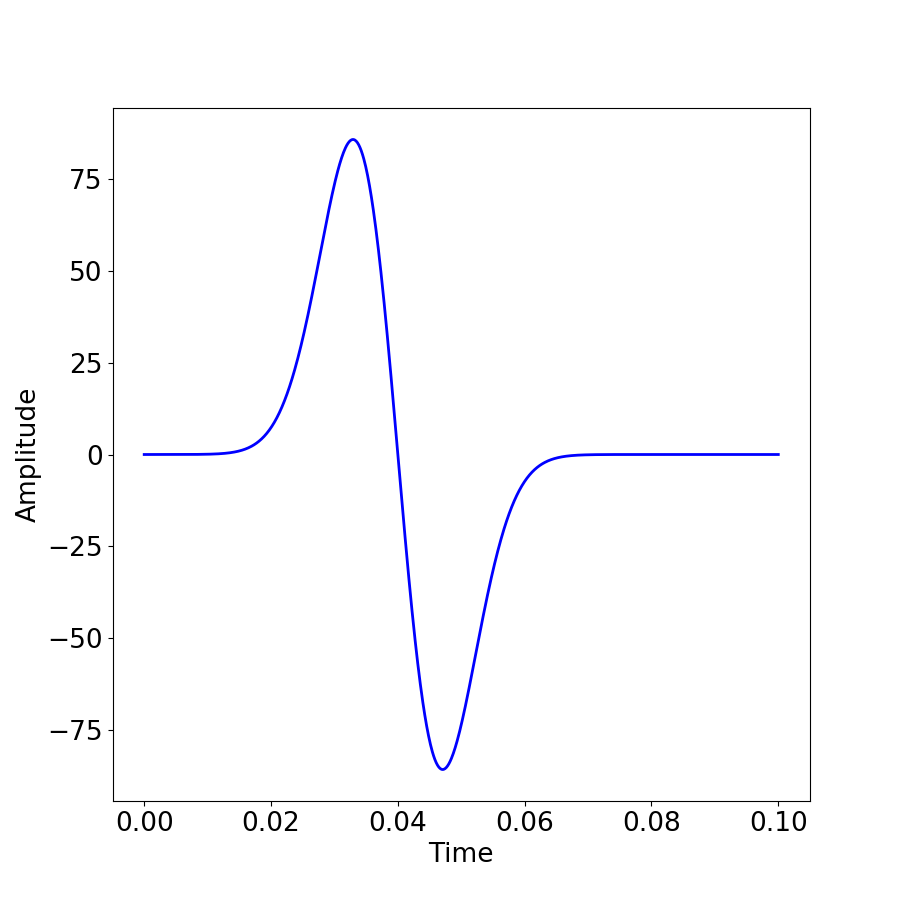
\includegraphics[width=80mm]{images/Source.png}
	\caption{Monopole source as a function of time}
\end{figure}
We enclose the monopole source using a cuboidal Kirchhoff surface whose diagonally opposite points are $p_{1} = (-1.0, -1.0, -1.0)$
and $p_{2} = (1.0, 1.0, 1.0)$. The surface is embedded in a cuboidal domain of size $[-5.0,5.0]\times[-5.0,5.0]\times[-5.0,5.0]$. The domain is discretized into structured grid of size $h = 0.1$ and the Kirchhoff surface is discretized into square cells of size $h = 0.1$. The pressure and its derivatives are interpolated from cell centers to quadrature points on Kirchhoff surface using fourth-order WENO polynomial. The Kirchhoff Integral (\ref{Kirchhoff Integral}) is computed using the two-point Gauss quadrature formula. The exact and numerical pressure are evaluated at observer point $xo = (3.0,3.0,3.0)$ and plotted against the function of time.
\begin{figure}[h!]\label{Result}
	\centering
	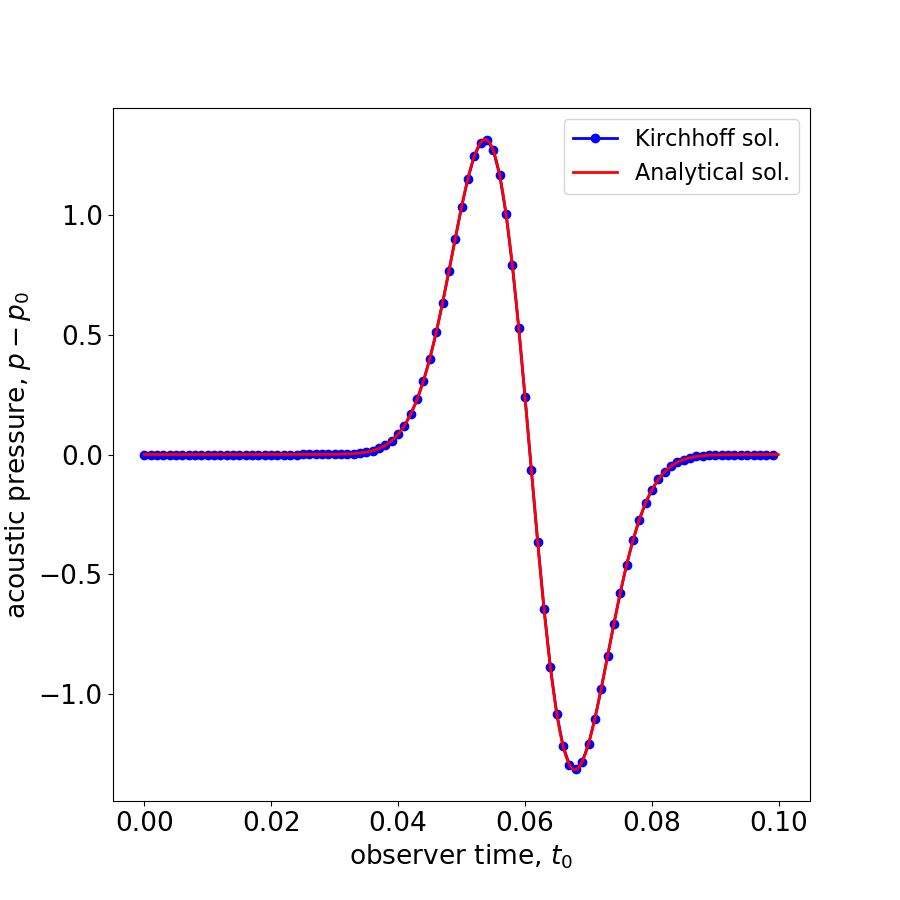
\includegraphics[width=80mm]{images/Pressure.png}
	\caption{The exact and numerical pressure as a function of time at observer point $xo = (3.0,3.0,3.0)$.}
\end{figure}
\subsection{Kirchhoff solver coupled with compressible Euler equation solver}
The goal of the test case is to validate the Kirchhoff solver by comparing the acoustic pressure computed using the Kirchhoff method and the flow solver at the observer point. We solve the compressible Euler equation
\begin{align}
	\frac{\partial \rho}{\partial t} + \nabla . (\rho \mathbf{u}) = 0,                                  \\
	\frac{\partial \rho \mathbf{u}}{\partial t} + \nabla . (\rho \mathbf{u} \mathbf{u}) + \nabla P	 = 0, \\
	\frac{\partial E}{\partial t} + \nabla . ((E + P) \mathbf{u}) = 0,                                  \\
	p = (\gamma - 1)(E - \frac{1}{2}\rho \mathbf{u}^{2}).
\end{align}
for an initial condition
\begin{align*}
	\rho       & = \rho_{0} + \rho',       \\
	\mathbf{u} & = 0,                      \\
	p          & = p_{0} + c_{0}^{2}\rho'.
\end{align*}
Where,
\[
	\rho'=
	\begin{cases}
		A \exp({-30r^{3}}), & \text{if } r\leq .125 \\
		0,                  & \text{otherwise}.
	\end{cases}
\]A = 0.01 is the amplitude of density perturbation and $r$ is the distance measured from center of the domain.
The ratio of the specific heat of the gas is $\gamma = 1.4$. The mean density and pressure of the gas are $\rho_{0} = 1.0$ and $p_{0} = 1.0$.
Then the speed of sound is given by $c_{0}= \sqrt{\frac{\gamma p_{0}}{\rho_{0}}} = 1.18321$.
We apply the transmissive boundary conditions in all the boundaries.
The compressible Euler equation is discretized using the finite-volume method.
We use the fourth-order WENO polynomial for spatial reconstruction
and SSPRK54 for temporal discretization. The flux is computed using LLF Riemann solver.
We discretize a domain of size $[0, 1] \times [0, 1] \times [0, 1]$  using $200 \times 200 \times 200$ cells. A CFL number of 0.9 is chosen for time discretization. The simulation is carried out for time $T = 1.0$.

We create a Kirchhoff box surface whose diagonally opposite points are $p_{1} = (0.195, 0.195, 0.195)$
and $p_{2} = (0.8, 0.8, 0.8)$. The surface is discretized using the square cells of size $h = 0.005$. We use fourth-order WENO polynomial to interpolate pressure data from cell centers to quadrature points on Kirchhoff surface. We use linear interpolation in time to compute pressure at emission time. The Kirchhoff Integral is computed using the two-point Gauss quadrature formula. The acoustic pressure $p' = p - p_{0}$ is computed at observer point $xo = (0.8975,0.8975,0.8975)$ and the observer time ranges from $t_{0} = [0,1.0]$ with time-step $dt = 0.01$.
\begin{figure}[h!]\label{result}
	\centering
	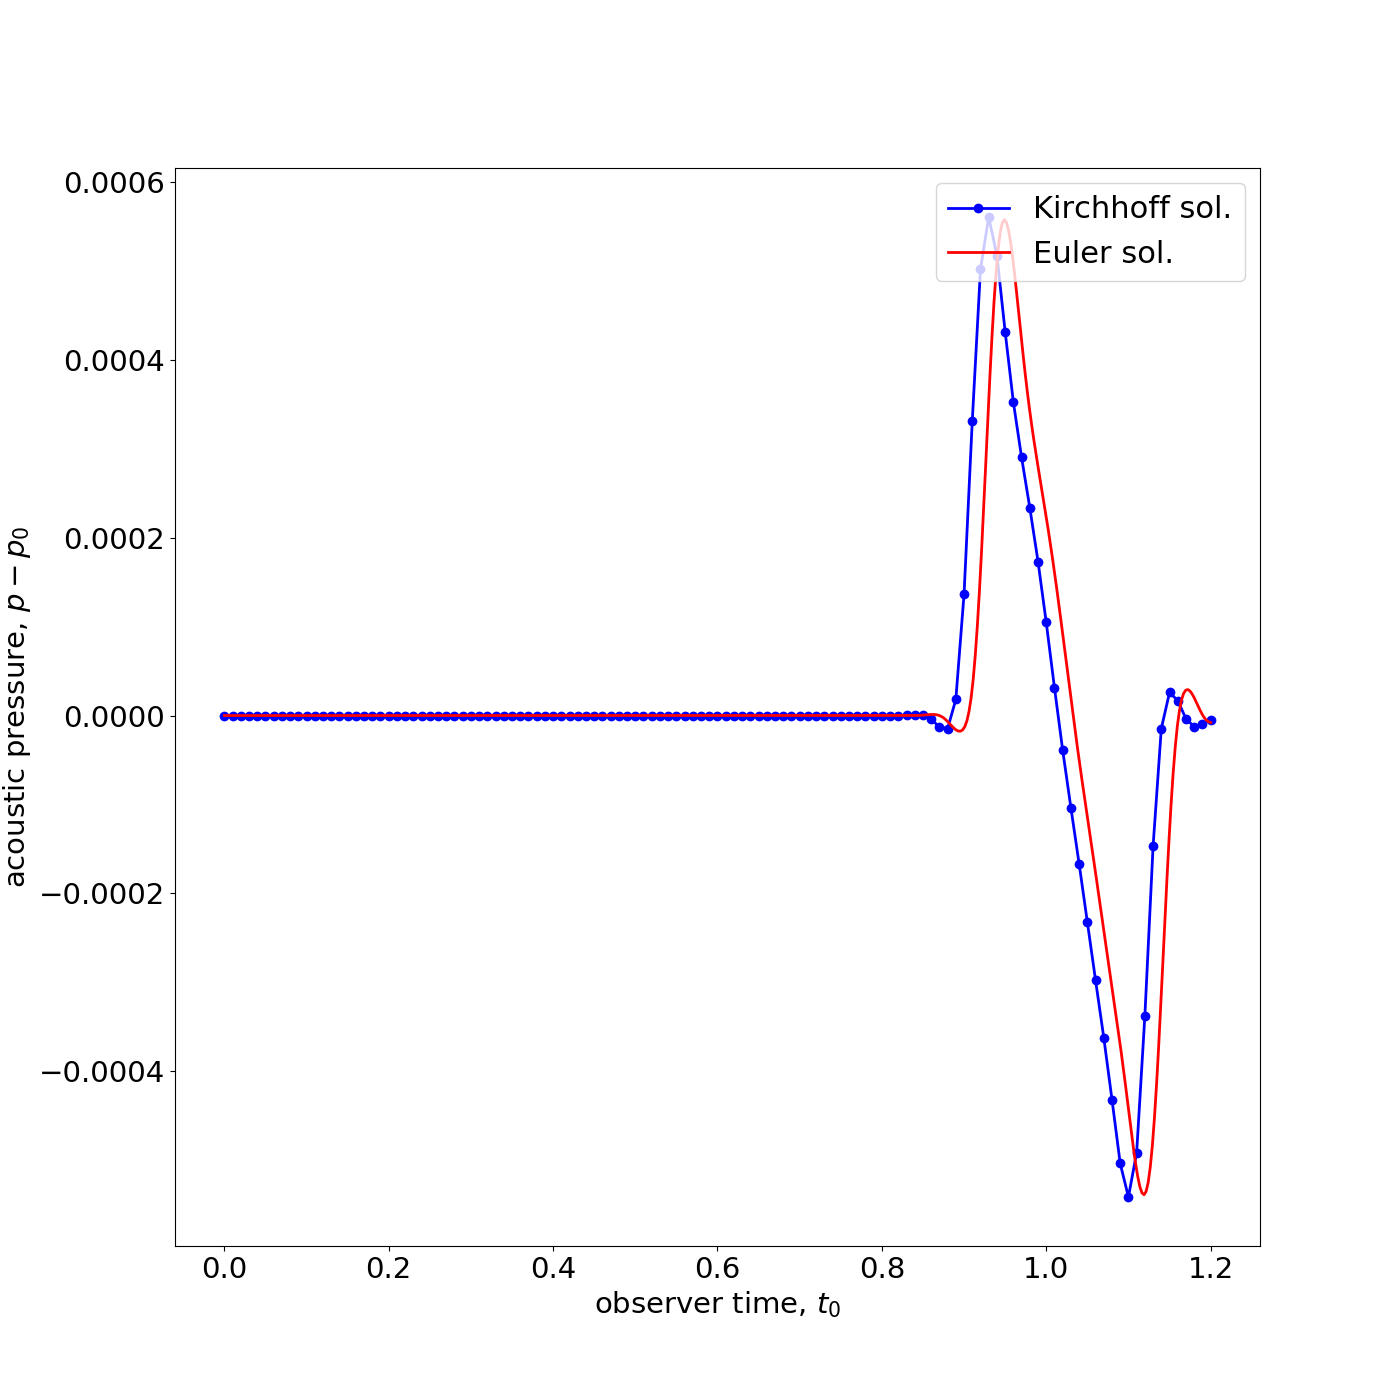
\includegraphics[scale=.23]{images/Pressure2.png}
	\caption{The acoustic pressure $p' = p - p_{0}$ is computed at observer point $x_{0}$ using Euler and Kirchhoff solver and plotted against observer time $t_{0}$.}
\end{figure}
\printbibliography
\end{document}


\printbibliography
\end{document}

